\chapter{Deployment on the Jetson Nano and Monitoring Interface}
\section{Introduction}
The final stage of the project involves deploying the trained winner models on the NVIDIA Jetson Nano platform, and 
developing a monitoring interface to visualize real-time system status and all the relevant information.

\section{Overview of the Jetson Nano}
The Jetson Nano is an entry‑level edge AI computer from NVIDIA, designed for low‑power embedded inference and light training.
Table~\ref{tab:jetson_nano_specs} summarises the specifications that are most relevant to the present work.
The board’s compact form factor (69.6 mm × 45 mm SO‑DIMM module) and 5–10 W power envelope make it suitable for deployment in resource‑constrained environments while still offering GPU‑accelerated computation\citep{jetson_specs}.
Figure~\ref{fig:jetson_components} provides a visual overview of the main hardware components in the Jetson Nano.

\begin{table}[H]
\centering
\caption{Key specifications of the NVIDIA Jetson Nano .}
\label{tab:jetson_nano_specs}
\begin{tabular}{@{}lc@{}}
\toprule
Component & Detail \\
\midrule
GPU & 128‑core NVIDIA Maxwell™, 472 GFLOPS (FP16) \\
CPU & Quad‑core ARM® Cortex®‑A57 @ 1.43 GHz \\
Memory & 4 GB 64‑bit LPDDR4, 25.6 GB/s \\
Video encode & 1× 4K30 (H.265), 2× 1080p60 (H.265) \\
Video decode & 1× 4K60, 4× 1080p60 (H.265) \\
Camera interface & Up to 4 cameras (12 lanes MIPI CSI‑2, 18 Gbps) \\
Connectivity & 1× Gigabit Ethernet, 1× USB 3.0, 3× USB 2.0 \\
Display & 1× DisplayPort 1.2 / 1× HDMI 2.0 \\
Power & 5–10 W \\
\bottomrule
\end{tabular}
\end{table}

\begin{figure}[H]
\centering
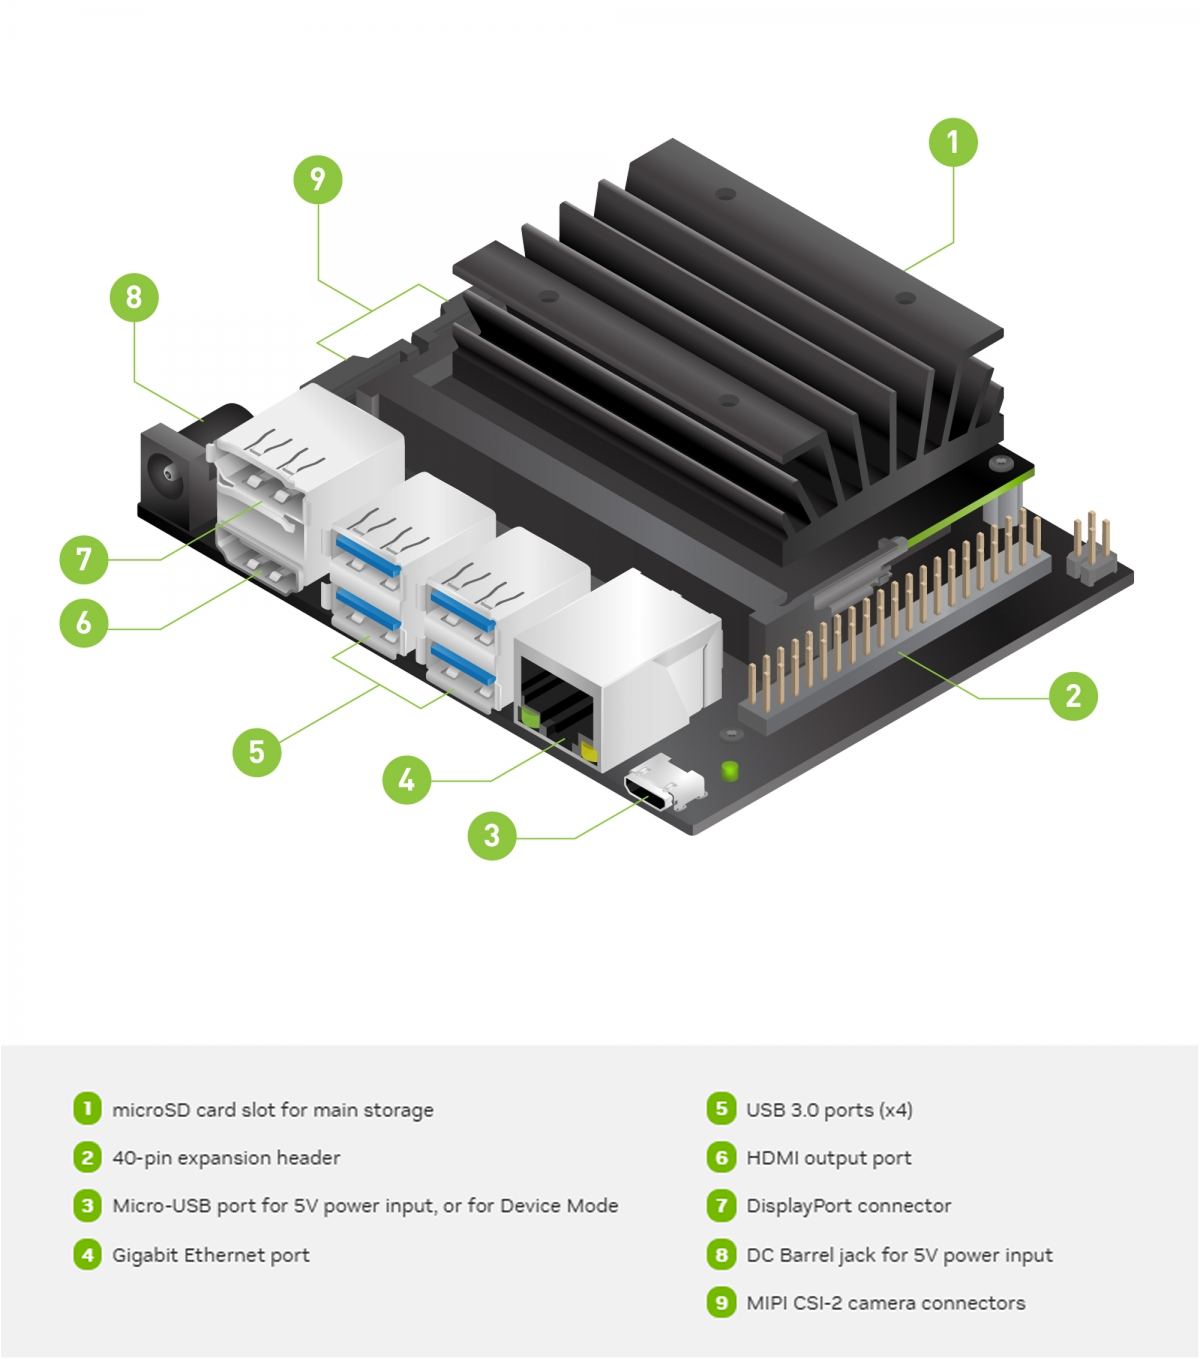
\includegraphics[width=0.6\textwidth]{figures/deployment/jetson-components.png}
\caption{Main components of the NVIDIA Jetson Nano developer kit used for edge deployment.}
\label{fig:jetson_components}
\end{figure}

The Jetson Nano runs a custom operating system image built by NVIDIA, known as Linux for Tegra (L4T), which is an Ubuntu 18.04‑based distribution specifically tailored for the Jetson hardware. This image ships with the JetPack SDK (version 4.x), providing a full development environment that includes CUDA 10, cuDNN, and TensorRT, all pre‑configured to leverage the Maxwell GPU. The kernel and device drivers are optimised for the Nano’s power management, multimedia engines, and camera interfaces, ensuring that the entire software stack—from low‑level sensor capture to GPU‑accelerated inference—can be executed without additional integration effort.

% The 128‑core Maxwell GPU delivers 472 GFLOPS of half‑precision performance, enabling real‑time inference of moderately sized neural networks.
% Combined with a quad‑core Cortex‑A57 CPU and 4 GB of fast LPDDR4 memory, the platform can execute the instrument recognition pipeline described in this thesis with low latency.
% Hardware‑accelerated H.265 encoding and decoding allow direct processing of high‑resolution video streams, while the MIPI CSI‑2 lanes and Gigabit Ethernet interface provide flexible options for camera integration and data transfer.
% The module’s 10 W maximum power draw makes it viable for continuous operation in a standalone embedded setting without active cooling.

\subsection{Limitations of the Jetson Nano}
While the Jetson Nano offers a compelling balance of performance, power efficiency and affordability. It comes with several
limitations that must be considered when deploying the models and developing the monitoring interface. Table \ref{tab:jetson_nano_limitations} summerizes the key constraints and their implications.

\begin{table}[H]
\centering
\caption{Limitations of the Jetson Nano and their practical implications.}
\label{tab:jetson_nano_limitations}
\begin{tabular}{@{}p{5cm}p{10cm}@{}}
\toprule
\textbf{Limitation} & \textbf{Implication} \\
\midrule
Limited storage and RAM & The deployed model and monitoring platform must be lightweight in both disk footprint and memory consumption; large models or extensive logging can exhaust storage, while memory‑intensive operations risk out‑of‑memory errors or performance degradation from swapping. \\
\midrule
Modest computing power & Models need to be compact and inference‑optimised (e.g., TensorRT engines, quantised formats) to achieve real‑time performance without overwhelming the processor. \\
\midrule
No active cooling (Heatsink Only) & Continuous temperature monitoring is essential to prevent throttling or hardware damage, especially under sustained GPU load in enclosures with limited airflow. \\
\midrule
Uncommon Architecture (aarch64) & Many third‑party libraries either lack official ARM64 builds or are distributed only as unofficial, potentially outdated, community‑maintained alternatives, complicating dependency management and reducing reliability. \\
\bottomrule
\end{tabular}
\end{table}

\section{Models Deployment on the Jetson Nano}




